% Options for packages loaded elsewhere
\PassOptionsToPackage{unicode}{hyperref}
\PassOptionsToPackage{hyphens}{url}
%
\documentclass[
  ignorenonframetext,
]{beamer}
\usepackage{pgfpages}
\setbeamertemplate{caption}[numbered]
\setbeamertemplate{caption label separator}{: }
\setbeamercolor{caption name}{fg=normal text.fg}
\beamertemplatenavigationsymbolsempty
% Prevent slide breaks in the middle of a paragraph
\widowpenalties 1 10000
\raggedbottom
\setbeamertemplate{part page}{
  \centering
  \begin{beamercolorbox}[sep=16pt,center]{part title}
    \usebeamerfont{part title}\insertpart\par
  \end{beamercolorbox}
}
\setbeamertemplate{section page}{
  \centering
  \begin{beamercolorbox}[sep=12pt,center]{part title}
    \usebeamerfont{section title}\insertsection\par
  \end{beamercolorbox}
}
\setbeamertemplate{subsection page}{
  \centering
  \begin{beamercolorbox}[sep=8pt,center]{part title}
    \usebeamerfont{subsection title}\insertsubsection\par
  \end{beamercolorbox}
}
\AtBeginPart{
  \frame{\partpage}
}
\AtBeginSection{
  \ifbibliography
  \else
    \frame{\sectionpage}
  \fi
}
\AtBeginSubsection{
  \frame{\subsectionpage}
}

\usepackage{amsmath,amssymb}
\usepackage{lmodern}
\usepackage{iftex}
\ifPDFTeX
  \usepackage[T1]{fontenc}
  \usepackage[utf8]{inputenc}
  \usepackage{textcomp} % provide euro and other symbols
\else % if luatex or xetex
  \usepackage{unicode-math}
  \defaultfontfeatures{Scale=MatchLowercase}
  \defaultfontfeatures[\rmfamily]{Ligatures=TeX,Scale=1}
\fi
\usetheme[]{defaultcustom2.scss}
% Use upquote if available, for straight quotes in verbatim environments
\IfFileExists{upquote.sty}{\usepackage{upquote}}{}
\IfFileExists{microtype.sty}{% use microtype if available
  \usepackage[]{microtype}
  \UseMicrotypeSet[protrusion]{basicmath} % disable protrusion for tt fonts
}{}
\makeatletter
\@ifundefined{KOMAClassName}{% if non-KOMA class
  \IfFileExists{parskip.sty}{%
    \usepackage{parskip}
  }{% else
    \setlength{\parindent}{0pt}
    \setlength{\parskip}{6pt plus 2pt minus 1pt}}
}{% if KOMA class
  \KOMAoptions{parskip=half}}
\makeatother
\usepackage{xcolor}
\newif\ifbibliography
\setlength{\emergencystretch}{3em} % prevent overfull lines
\setcounter{secnumdepth}{-\maxdimen} % remove section numbering


\providecommand{\tightlist}{%
  \setlength{\itemsep}{0pt}\setlength{\parskip}{0pt}}\usepackage{longtable,booktabs,array}
\usepackage{calc} % for calculating minipage widths
\usepackage{caption}
% Make caption package work with longtable
\makeatletter
\def\fnum@table{\tablename~\thetable}
\makeatother
\usepackage{graphicx}
\makeatletter
\def\maxwidth{\ifdim\Gin@nat@width>\linewidth\linewidth\else\Gin@nat@width\fi}
\def\maxheight{\ifdim\Gin@nat@height>\textheight\textheight\else\Gin@nat@height\fi}
\makeatother
% Scale images if necessary, so that they will not overflow the page
% margins by default, and it is still possible to overwrite the defaults
% using explicit options in \includegraphics[width, height, ...]{}
\setkeys{Gin}{width=\maxwidth,height=\maxheight,keepaspectratio}
% Set default figure placement to htbp
\makeatletter
\def\fps@figure{htbp}
\makeatother

\makeatletter
\makeatother
\makeatletter
\makeatother
\makeatletter
\@ifpackageloaded{caption}{}{\usepackage{caption}}
\AtBeginDocument{%
\ifdefined\contentsname
  \renewcommand*\contentsname{Table of contents}
\else
  \newcommand\contentsname{Table of contents}
\fi
\ifdefined\listfigurename
  \renewcommand*\listfigurename{List of Figures}
\else
  \newcommand\listfigurename{List of Figures}
\fi
\ifdefined\listtablename
  \renewcommand*\listtablename{List of Tables}
\else
  \newcommand\listtablename{List of Tables}
\fi
\ifdefined\figurename
  \renewcommand*\figurename{Figure}
\else
  \newcommand\figurename{Figure}
\fi
\ifdefined\tablename
  \renewcommand*\tablename{Table}
\else
  \newcommand\tablename{Table}
\fi
}
\@ifpackageloaded{float}{}{\usepackage{float}}
\floatstyle{ruled}
\@ifundefined{c@chapter}{\newfloat{codelisting}{h}{lop}}{\newfloat{codelisting}{h}{lop}[chapter]}
\floatname{codelisting}{Listing}
\newcommand*\listoflistings{\listof{codelisting}{List of Listings}}
\makeatother
\makeatletter
\@ifpackageloaded{caption}{}{\usepackage{caption}}
\@ifpackageloaded{subcaption}{}{\usepackage{subcaption}}
\makeatother
\makeatletter
\@ifpackageloaded{tcolorbox}{}{\usepackage[many]{tcolorbox}}
\makeatother
\makeatletter
\@ifundefined{shadecolor}{\definecolor{shadecolor}{rgb}{.97, .97, .97}}
\makeatother
\makeatletter
\makeatother
\ifLuaTeX
  \usepackage{selnolig}  % disable illegal ligatures
\fi
\IfFileExists{bookmark.sty}{\usepackage{bookmark}}{\usepackage{hyperref}}
\IfFileExists{xurl.sty}{\usepackage{xurl}}{} % add URL line breaks if available
\urlstyle{same} % disable monospaced font for URLs
\hypersetup{
  pdftitle={Slides for classroom communication},
  pdfauthor={CTTI, goAJK Sep 20, 2022},
  hidelinks,
  pdfcreator={LaTeX via pandoc}}

\title{{Slides for classroom communication}}
\author{{CTTI, goAJK}{Sep 20, 2022}}
\date{}
\logo{\includegraphics{logo\_soe.jpg}}

\begin{document}
\frame{\titlepage}
\ifdefined\Shaded\renewenvironment{Shaded}{\begin{tcolorbox}[frame hidden, interior hidden, boxrule=0pt, sharp corners, enhanced, breakable, borderline west={3pt}{0pt}{shadecolor}]}{\end{tcolorbox}}\fi

\hypertarget{if-we-want-to-move-from-a-future-we-dont-want-to-a-future-we-wantwe-have-to-consciously-practice-bold-thinking-to-achieve-the-desired-future.}{%
\section{If we want to move from a future we dont want to a future we
want,we have to consciously practice bold thinking to achieve the
desired
future.}\label{if-we-want-to-move-from-a-future-we-dont-want-to-a-future-we-wantwe-have-to-consciously-practice-bold-thinking-to-achieve-the-desired-future.}}

\begin{frame}{
\includegraphics[width=13.54167in,height=7.8125in]{images/mandela.jpg}}
\protect\hypertarget{section}{}
\end{frame}

\begin{frame}{About Me}
\protect\hypertarget{about-me}{}
\begin{columns}[T]
\begin{column}{0.3\textwidth}

\includegraphics[width=6.25in,height=\textheight]{images/zahid.jpg}
\end{column}

\begin{column}{0.7\textwidth}
\begin{itemize}
\tightlist
\item
  Ph.D (Economics) --- Pakistan Institute of Development Economics, 2007
\item
  MSc (Statistics)
\item
  Specializations:

  \begin{itemize}
  \tightlist
  \item
    Applied Econoetrics
  \item
    Data Analyst
  \item
    Development Economics
  \end{itemize}
\item
  Research interests : data for policy, data and analytical skill
  development ,data for policy
\end{itemize}
\end{column}
\end{columns}
\end{frame}

\hypertarget{how-to-give-a-killer-presentation-hbr}{%
\section{\texorpdfstring{\href{https://hbr.org/2013/06/how-to-give-a-killer-presentation}{How
to Give a Killer Presentation
HBR}}{How to Give a Killer Presentation HBR}}\label{how-to-give-a-killer-presentation-hbr}}

\begin{frame}{Why do we teach?}
\protect\hypertarget{why-do-we-teach}{}
\begin{itemize}[<+->]
\item
  \textbf{What is your mission of teaching?}
\item
  \textbf{What is happening when we teach?}
\item
  \textbf{What is teaching?}
\end{itemize}
\end{frame}

\begin{frame}{}
\protect\hypertarget{section-1}{}
\end{frame}

\begin{frame}{}
\protect\hypertarget{section-2}{}
\end{frame}

\begin{frame}{Contents:}
\protect\hypertarget{contents}{}
\begin{enumerate}[<+->]
\item
  \textbf{Requirements of a good teacher}
\item
  \textbf{Types of Teacher}
\item
  \textbf{Lecturing}
\item
  \textbf{Requirements of Successful Lecturing}
\item
  \textbf{Oral presentation Material and Methods}
\item
  \textbf{Requirements of Ideal effective lecturing}
\item
  \textbf{Characteristics of Good Instructions.}
\end{enumerate}
\end{frame}

\begin{frame}{}
\protect\hypertarget{section-3}{}
\begin{enumerate}[<+->]
\setcounter{enumi}{7}
\item
  \textbf{Structure of the lecture}
\item
  \textbf{Summary of the requirements for an ideal and effective
  lecture}
\item
  \textbf{Closure}
\item
  \textbf{Summary}
\item
  \textbf{Conclusion}
\end{enumerate}
\end{frame}

\begin{frame}{Good Teacher}
\protect\hypertarget{good-teacher}{}
\begin{block}{good teacher}
\protect\hypertarget{good-teacher-1}{}
\begin{figure}

{\centering 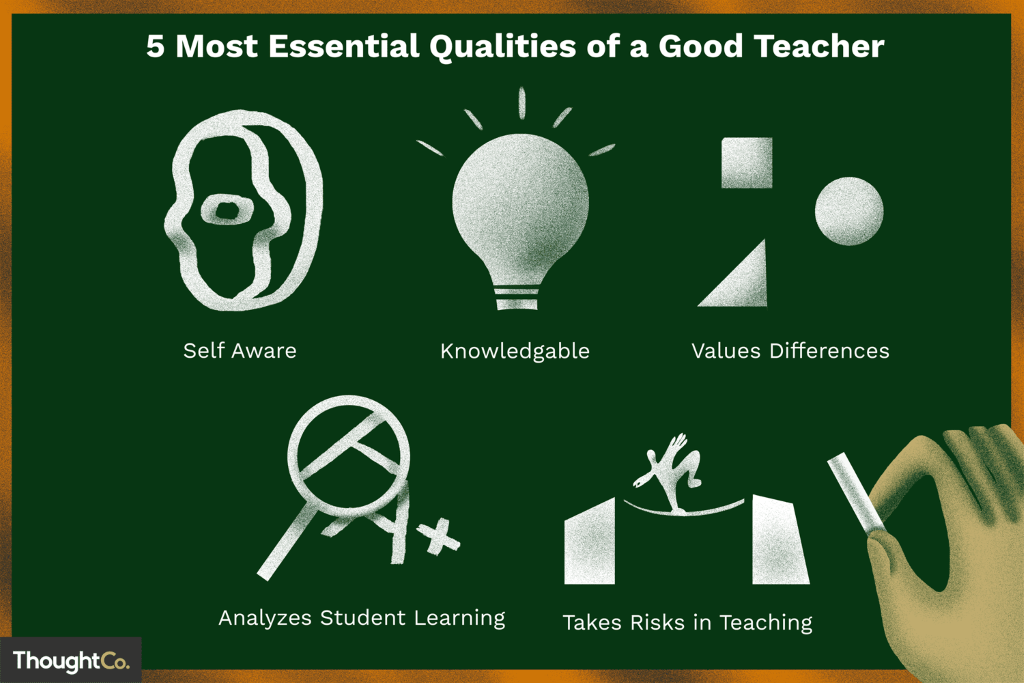
\includegraphics[width=7.30208in,height=\textheight]{images/good_teacher.png}

}

\end{figure}
\end{block}

\begin{block}{How to become a good teacher?}
\protect\hypertarget{how-to-become-a-good-teacher}{}
\begin{figure}

{\centering 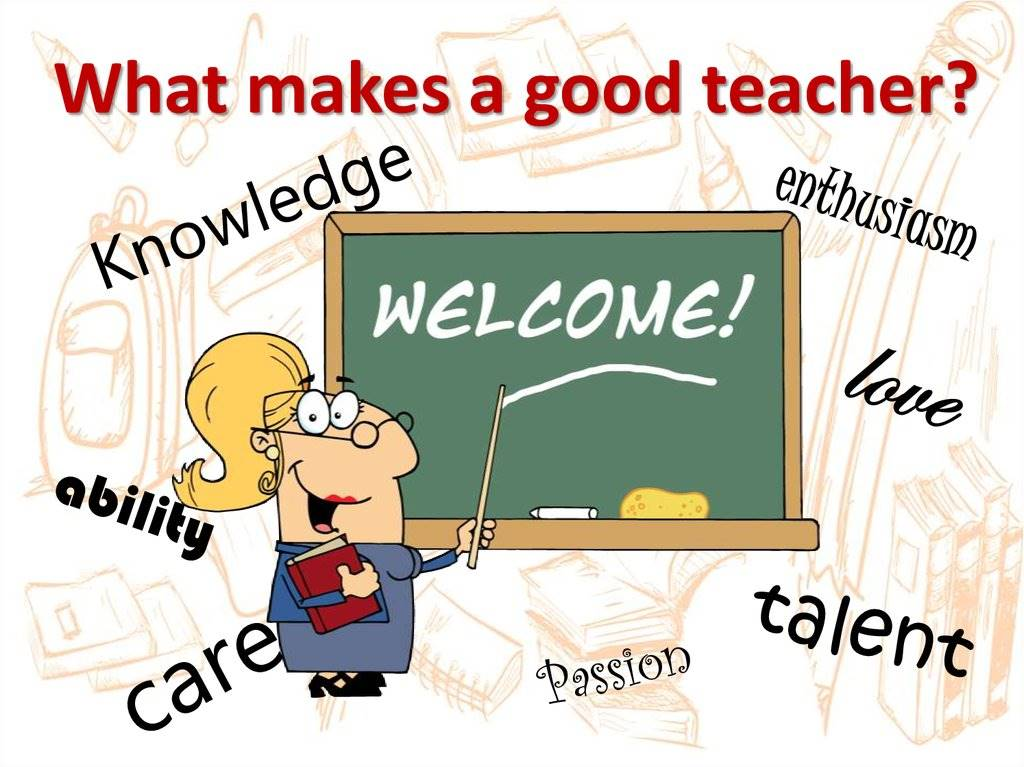
\includegraphics[width=7.04167in,height=\textheight]{images/good_teacher1.jpg}

}

\end{figure}
\end{block}
\end{frame}

\begin{frame}{Modes of communication}
\protect\hypertarget{modes-of-communication}{}
\begin{itemize}[<+->]
\item
  {\textbf{Verbal}} \textbf{-- speaking words. Voice tone/pitch/volume.}
\item
  \textbf{Intonation : sarcastic, sad Word choice : lecture , friends ,
  scientific meeting,}
\item
  {\textbf{Nonverbal}} \textbf{: Knowledge ,skill \& eye contact ,. body
  language, facial expression , gestures.}
\item
  {\textbf{Written Communication ; Explain ?}}
\end{itemize}
\end{frame}

\begin{frame}{Types of Teachers}
\protect\hypertarget{types-of-teachers}{}
\begin{itemize}[<+->]
\tightlist
\item
  \textbf{A mediocre Teacher : Tells}
\item
  {\textbf{A good Teacher : explains}}
\item
  \textbf{A superior Teacher : demonstrates}
\item
  {\textbf{A great Teacher : inspires}}
\item
  \textbf{A great Teacher uses : E C M T}
\item
  {\textbf{(}}\textbf{E{ffective} C{lassroom} M{anagement}
  T{echniques})}
\end{itemize}
\end{frame}

\begin{frame}{\href{pollev.com}{polleverywhere}}
\protect\hypertarget{polleverywhere}{}
\href{https://pollev-embeds.com/free_text_polls/lMfTtIjDiyJAdppRzvQbb}{An
ideal teacher}

\note{World is changing rapidly

luck and preparedness

daily microgains

average life

commitment, conviction, consistency, clarity}
\end{frame}

\begin{frame}{Lecturing}
\protect\hypertarget{lecturing}{}
\begin{block}{is a process by which knowledge is transferred from the
teacher {(expert)} to young learners{(students)}. Unfortunately, there
is {no single magical formula} for that but still quite possible by
following a series of steps and procedures which I hope will be made
part of this training.}
\protect\hypertarget{is-a-process-by-which-knowledge-is-transferred-from-the-teacher-expert-to-young-learnersstudents.-unfortunately-there-is-no-single-magical-formula-for-that-but-still-quite-possible-by-following-a-series-of-steps-and-procedures-which-i-hope-will-be-made-part-of-this-training.}{}
\end{block}
\end{frame}

\begin{frame}{}
\protect\hypertarget{section-4}{}
\textbf{Lecturer job:lessen student fears and encourage students to
pursue deeper understanding}

a- {These include several teaching and curriculum approaches that can be
integrated into typical quantitative methods classes.}

b- integration during the class;

\begin{itemize}[<+->]
\item
  expanded opportunities for two-way communication;
\item
  developing co-ownership of the course along with the students;
\item
  alternating lecture with small-group work to aid in learning difficult
  topics.
\end{itemize}
\end{frame}

\begin{frame}{Poor slide}
\protect\hypertarget{poor-slide}{}
\begin{itemize}[<+->]
\item
  {\textbf{\emph{Some students seem naturally enthusiastic about
  learning, but many need-or expect-their instructors to inspire,
  challenge, and stimulate them:}}}
\item
  {\textbf{\emph{``Effective learning in the classroom depends on the
  teacher's ability \ldots{} ??}}}
\end{itemize}
\end{frame}

\begin{frame}{Favorable classroom atmosphere}
\protect\hypertarget{favorable-classroom-atmosphere}{}
\begin{itemize}[<+->]
\item
  \textbf{Some students seem naturally enthusiastic about learning, but
  many need-or expect-their instructors to {inspire, challenge, and
  stimulate} them:}
\item
  {\textbf{``Effective learning in the classroom depends on the
  teacher's ability \ldots{} ??}}
\end{itemize}
\end{frame}

\begin{frame}{Teaching Modules}
\protect\hypertarget{teaching-modules}{}
\begin{itemize}[<+->]
\item
  a-\textbf{Improving teaching provision within the department by
  identifying models of best practice and promoting new teaching
  initiatives and curriculum development.}
\item
  b- \textbf{Promote links with other departments and/or disciplines
  where possible.}
\item
  {\textbf{Trans-disciplinary and multidisciplinary}}
\end{itemize}
\end{frame}

\begin{frame}{Interactive Learning}
\protect\hypertarget{interactive-learning}{}
\textbf{Course assessment}

\textbf{Students assessment}

{\textbf{Teaching Methods}}

A thousand teachers,

a thousand methods.(Chinese proverb)
\end{frame}

\begin{frame}{Oral Presentation: Methods and Materials}
\protect\hypertarget{oral-presentation-methods-and-materials}{}
\begin{enumerate}[<+->]
\item
  {YOUR VOICE}( audibility, pitch, pronunciation, pause. tone?.) How do
  you relieve monotony in your lecture?
\item
  {BODY LANGUAGE}(Gestures ,pacing but no unpleasant movements)
\item
  {APPEARANCE} (posture , .freezing in one corner?)
\item
  {Speed}
\end{enumerate}
\end{frame}

\begin{frame}{Effective Presentation}
\protect\hypertarget{effective-presentation}{}
\href{https://www.branchtrack.com/projects/bv28y7r3}{Effective
Presentation} 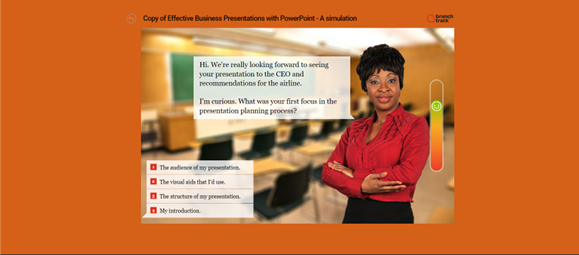
\includegraphics{images/presentation_sim.png}
\end{frame}

\hypertarget{how-to-beat-death-by-powerpoint}{%
\section{How to beat death by
powerpoint}\label{how-to-beat-death-by-powerpoint}}

\begin{frame}{Closure}
\protect\hypertarget{closure}{}
\begin{enumerate}[<+->]
\tightlist
\item
  \textbf{No single teaching method covers everything}
\item
  \textbf{Optimal approach features a mixture of instructional methods
  and learning activities}
\item
  \textbf{Optimal mixture changes over time with change in students?}
\item
  \textbf{Students involvement in the learning process}
\item
  \textbf{Favorable classroom environment}
\end{enumerate}
\end{frame}

\begin{frame}{Summary}
\protect\hypertarget{summary}{}
\begin{itemize}[<+->]
\item
  {\textbf{What one thing did you learn today?}}
\item
  \textbf{How does today's lesson impact your understanding?}
\item
  {\textbf{How would you summarize today's lecture for someone who
  wasn't here?}}
\item
  \textbf{What was the most significant learning from today's lecture?}
\item
  {\textbf{What was the most difficult concept in today's lecture?}}
\item
  \textbf{What should I review further in our next lecture?}
\item
  {\textbf{What was one thing you were unsure about in the lecture ?}}
\item
  \textbf{Clarify areas of confusion}
\end{itemize}
\end{frame}

\hypertarget{the-ability-to-learn-faster-than-your-competitors-may-be-the-only-sustainable-competitive-advantage1}{%
\section[The ability to learn faster than your competitors may be the
only sustainable competitive advantage]{\texorpdfstring{The ability to
learn faster than your competitors may be the only sustainable
competitive
advantage\footnote<.->{Peter Senge: The Fifth Discipline}}{The ability to learn faster than your competitors may be the only sustainable competitive advantage}}\label{the-ability-to-learn-faster-than-your-competitors-may-be-the-only-sustainable-competitive-advantage1}}

\begin{frame}{}
\protect\hypertarget{section-5}{}
\begin{columns}[T]
\begin{column}{0.3\textwidth}
\includegraphics{images/gr8_teacher.webp}\href{https://owlcation.com/academia/Characteristics-Of-A-Good-Teacher}{What
makes a great teacher? A brief summary}
\end{column}

\begin{column}{0.7\textwidth}
\begin{itemize}[<+->]
\tightlist
\item
  Expert communication skills
\item
  Superior listening skills
\item
  Deep knowledge and passion for their subject matter
\item
  The ability to build caring relationships with students
\item
  Friendliness and approachability
\item
  Excellent preparation and organization skills
\item
  Strong work ethic
\item
  Community-building skills
\item
  High expectations for all
\end{itemize}
\end{column}
\end{columns}
\end{frame}

\begin{frame}{Digital era education: challenges and oppotunities}
\protect\hypertarget{digital-era-education-challenges-and-oppotunities}{}
\begin{itemize}[<+->]
\tightlist
\item
  \href{khanacademy.com}{Immense learning sources}
\item
  \href{youtube.com}{youtube} and
\item
  much more
\item
  \href{https://galtonboard.com/}{Galton Board}
\item
  \href{https://phet.colorado.edu/sims/html/plinko-probability/latest/plinko-probability_en.html}{Plinko}
\item
  Flip based class room teaching
\end{itemize}
\end{frame}

\begin{frame}{}
\protect\hypertarget{section-6}{}
\href{https://www.youtube.com/watch?v=UCFg9bcW7Bk}{Teaching methods for
inspiring students of the future}

\begin{itemize}[<+->]
\item
  ``\textbf{The mind is not a vessel that needs filling, but wood that
  needs igniting.}'' Plutarch AD46-AD120
\item
  ``\textbf{Education is not the learning of facts, but the training of
  the mind to think.}'' Abert Einstein 1879-1955
\end{itemize}
\end{frame}

\begin{frame}{}
\protect\hypertarget{section-7}{}
\textbf{Allow students to engage in:}

\begin{itemize}[<+->]
\item
  \textbf{Choice}
\item
  \textbf{Collaboration}
\item
  \textbf{Communication}
\item
  \textbf{Critical Thinking}
\item
  \textbf{Creativity} and {\textbf{greatest of all these is}}
\item
  {\textbf{LOVE}}
\end{itemize}
\end{frame}

\hypertarget{stay-hungry-stay-foolish}{%
\section{\texorpdfstring{{Stay Hungry, Stay
Foolish}}{Stay Hungry, Stay Foolish}}\label{stay-hungry-stay-foolish}}

\begin{frame}{}
\protect\hypertarget{section-8}{}
{I \emph{am a great} TEACHER}

{BECAUSE\ldots{}}
\end{frame}

\begin{frame}{Great teacher}
\protect\hypertarget{great-teacher}{}
\begin{itemize}[<+->]
\tightlist
\item
  {Celebrate mistakes}
\item
  {Appreciate differences}
\item
  {Relay feedback}
\item
  {Evaluate themselves}
\end{itemize}

\begin{quote}
\textbf{``{I have learned that people will forget what you}{said}},
{[}people will forget what you{]} {\textbf{did}}, {but people will never
forget how you made them} {\textbf{feel}}.'' -Maya Angelou
\end{quote}
\end{frame}



\end{document}
